\chapter{Implementation} \label{implementation}
Chapter \ref{design} gave an overview about the contents of the prototype application. The requirements as well as the storyline were set. Also, there was a look at how the provided hardware can be used for user interactions in the application. The chapter mentioned the different stakeholders and their tasks and requirements. This chapter will take a look at the application from the developer stakeholder role. It is a documentation of the development process of the VR application. There will be an introduction to the hardware and software tools from a technical point of view. The software architecture will be described as well as problems which occurred during the development and their solutions.

\section{Software development kits for VR applications} \label{sdksupport}
To develop mobile games and applications in VR which are compatible with the Samsung Gear VR there are different third party libraries or software development kits (SDKs) to support VR integration. The official partner of the Samsung Gear VR is Occulus, which provides several free SDK support libraries for mobile VR. First of all, A distinction must be drawn between the native SDKs and the game engine SDKs.\\
The native SDK is a support library for native Android applications. Developing native Android applications is more rudimentary and labour-intensive than developing with a game engine. Also the application can be optimised in performance and customization \cite{Occulus.2019}. Game engines on the other hand are a collection of different tools useful for game development combined in one software product. Different tasks like programming, game design, animation or graphics can be done within a game engine. A lot of work is automated in a game engine when it comes to developing games. \cite{?}\\
Occulus provides SDKs for the two game engines Unity and Unreal. Both are very commonly used game engines. For the development of the VR prototype application, Unity is chosen. The reasons for that are explained in the following chapter.

\section{Overview about Unity}
Unity is a multi platform game engine. Just as described before, a game engine helps to maintain different tasks which occur when developing a game under the shelter of one single platform. 
For the development of this prototype VR application, the game engine Unity and the Occulus Unity SDK is used. Unity is the preferred game engine, because it is beginner friendly and free for personal and academic use. Another positive aspect of Unity is the large community from hobby game developers to professional teams. The unity asset store provides many 3D objects, support libraries, textures, audios and other useful tools for game development. This so called assets can be imported into the engine very easily. There is a variety of free assets as well as paid assets. TODO: List other reasons why use unity asset store, community, object orientated programming language. \url{https://sundaysundae.co/unity-vs-unreal/}\\
\subsection{Unity Editor}
The Unity editor is the main too, which is used while creating the prototype. In the editor, game objects can be modified, the game can be compiled and tested. The editor view is organized in smaller windows which can be rearranged and each covers a functionality. The most important windows are the scene view, the inspector view, the game view and the hierarchy view. Figure \ref{fig:unity-editor} shows a screenshot of the unity editor and the different windows attached to it. In the top left corner there is the scene view with the game view underneath. The middle top window shows the hierarchy view. The right column is the inspector view. In the following the main functionalities of the views are described:
\paragraph{Scene view}
In the scene view, game objects can be placed, relocated and modified in the game scene. Game obejcts in unity are a very important concept. They can be 3D world objects, lights, cameras and special effects. A game object can also be seen as a container which can contain other game objects. The scene view is the most important view in the Unity editor, because from there, the whole look of the game scene is defined.
\paragraph{Inspector view}
The inspector view shows the details of a selected component. From there, the the detail properties of the objects can be seen and components can be attached and modified. A component in unity defines a specific property and always belongs to a game object. Every game object can have a variety of components attached. Components can change the appearance and behaviour of a game object in the game. There are several build in components available in unity, but through the scripting API it is possible to create highly customisable components. The inspector gives an overview about all components of the selected game object. New components can be attached in this view, and existing components can be deleted or modified.
\paragraph{Hierarchy view}
The hierarchy view gives an overview about all game objects in the scene in a structural tree diagram. Game objects selected in the hierarchy view get selected automatically in the scene view. During the development of the game, more and more game objects will be created for the scene. The hierarchy view is important to keep an overview about the game object and to group and reorganise the existing objects. It is possible to drag game objects from the hierarchy view to a specific prefab folder. Once a game object is in that folder it becomes a prefab, that means the game object can be reused within different scenes and even different projects.
\paragraph{Game view}
The game view shows a preview of the outcome for the game. It is a view rendered from the camera objects in the game. It is possible to run the game via the editor to see the outcome of modified components and test the game workflow. It is also possible to make temporary changes during the game is running in the editor to see the outcome in the game view.
\begin{figure}[h!]
  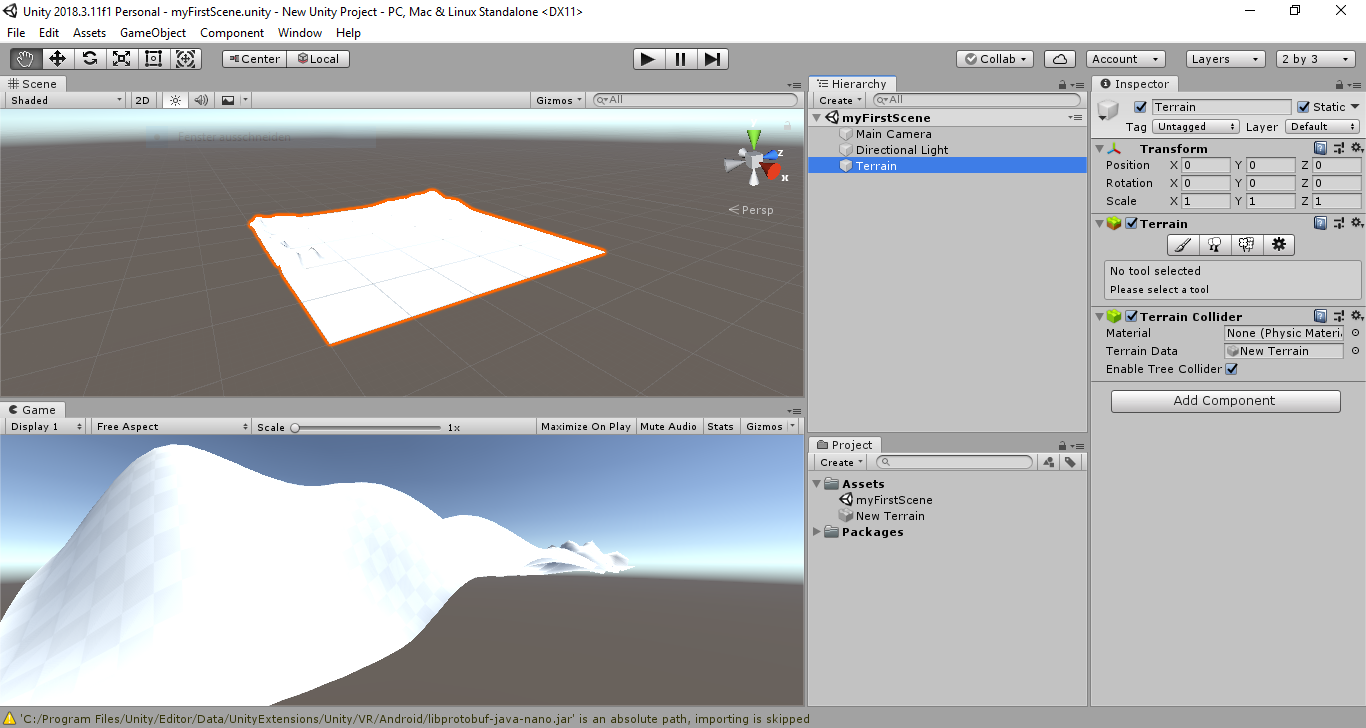
\includegraphics[width=16cm]{kapitel/editor.PNG}
  \centering
  \caption{Screenshot of Unity editor}
  \label{fig:unity-editor}
\end{figure}
\subsection{Scripting in Unity}
Unity provides a variety of predefined components, which can be attached to game objects, such as a Rigidbody for physical behaviour or an Audio source for playing music. However, for customizing the behaviour of a game object, it is possible to create components and attach a script to it. A script can either be written in C\# or a  modified JavaScript by Unity. For this prototype application, C\# is chosen, because it is the wider used programming language within the Unity community. Every component is a class and inheritates from the MonoBehaviour class. Through the scripting API all existing game objects and their components can be accessed and modified, it is possible to create new game objects, react to events, load new scenes and control the game flow. The MonoBehaviour class contains several methods which can be overwritten to execute code at some different lifecycle events. The update method for example is called every frame update of the game object. It can be used for example to get continues updated values from the game object. The start method is called once before the gameplay starts. This method is mostly used for initialization of other game objects or components.\\
In general, all rules, best practices and design patterns which are common in the .NET environment can be used within Unity as well. Unity uses some special concept of dependency injection, which is very important and will be explained shortly because it is often used in the prototype application: Every object variable which has public access in a class will be visible in the component in the inspector view. It is now possible to inject a reference to that variable by drag and drop a game object or a component to the variable in the inspector view. There is no need to initialize the variable in the code. Public primitive variables can also be modified through the inspector view.
\subsection{Unity and Samsung Gear VR support}
\todo{describe registering device}
In Unity, VR support can simply be enabled by ticking a box in the player settings. However, to make a game which is compatible with the Samsung Gear VR, more work than that has to be done. First of all, the Occulus support library has to be imported. It can be downloaded from the Unity asset store. This library is shortly introduced in chapter \ref{sdksupport} and contains a variety of components and prefabs. For this prototype the OVRCharacterController prefab from the SDK is used. It contains all necessary scripts and objects for the communication between Unity and the VR hardware. The OVRCharacterController is a first person controller which can be used in the VR environment. With the use of this prefab it is also easy to set up the Samsung Gear VR handheld controller support. The prefab contains a script called OVRInput which can register connected controllers and input events. However, the OVRCharacterController prefab is missing a handheld controller representation within the game. The user needs this kind of representation in order to see the movements of their hand while playing the game. Occulus provides a handheld controller game object. This object simply has to be attached to the OVRCharacterController prefab. Once the controller object is attached, the movements of the user's hand get automatically mapped to the virtual controller in the game. To realize selecting and object manipulation with this handheld controller, more adaptions have to be done. How this is solved is described in chapter \ref{inputmethods}.

\section{Scene design of different scenes}
Before starting to program the game logic, the outlook of the scenes has to be designed. This is an important step in the implementation because the look of the environment defines a first impression and is a factor when it comes to immersion. The more realistic the environment is designed, the more present users feel in the virtual world.
\subsection{Skyboxes}
Skyboxes are a concept in unity to design the background of the game. They are wrapped around the scene and give an impression of a wider environment. Mostly a skybox contains a 360 degree image. When moving around in a virtual world, the skybox image does not come closer, just as a horizon in a real environment.\\
For the prototype, an image with an urban environment is chosen. The image is a 360 photography of a place in a city surrounded by skyscrapers (TODO image). This image gets attached to the skybox component of the main camera. The image is used in all scenes, the world scene as well as the different laboratory scenes, to state out that the user has not left the city.
\subsection{World scene design}

\subsection{Software engineer scene design}
\section{VR specific problems}
\subsection{Input methods with Samsung Gear VR controller} \label{inputmethods}
\subsection{Implementation of the dialogue system}
\subsection{User guidance}